\chapter{Quadro Terminal para Painel Led 4x4}

Este capítulo mostra os valores efetivos para a confecção do quadro para o Painel LED Full Color. Foram usados os métodos de dimensionamento explicados no Capítulo \ref{cap:calculos}. Nas próximas seções, serão apresentados os parâmetros de projeto utilizados, a tabela de carga, os diagramas unifilar e multifilar e uma representação gráfica do quadro (esquema funcional) nas opções simples. Ao final, há uma lista de materiais para montagem.

\section{Parâmetros de projeto}

O Painel Full Color Led 4x4 é composto por 16 gabinetes e deve ser alimentado com 6 cabos de força. Há três opções de resolução (P10, P8 e P5), cada uma com sua potência. A Tabela \ref{tab:pot_4x4} apresenta as informações de potência de cada gabinete, a quantidade de cabos ou grupos de até 3 gabinetes para conectar à rede elétrica e a quantidade de gabinetes e a potência total do Painel.

\begin{table}[htbp]
\caption{Potência Painel LED 4x4}
\centering
\begin{tabular}{cccccc}
\toprule
\multirow{2}{*}{Item} & \multirow{2}{*}{Tipo} & \multirow{2}{*}{Potência (W)} & \multicolumn{3}{c}{Painéis} \\
\cmidrule{4-6}
& & & Cabos  & Gabinete & Potência Total (W) \\
\midrule


28 & P10 & 540 & 6 & 16 & 8640 \\
29 & P8 & 630 & 6 & 16 & 10080 \\
30 & P5 & 684 & 6 & 16 & 10944 \\


\bottomrule
\end{tabular}
\label{tab:pot_4x4}
\end{table}



\section{Tabela de Carga}
\section{Diagrama Unifilar}

\subsection{Trifásico 127/220 V}

\subsection{Trifásico 127/220 V}

\section{Diagrama Multifilar}

\subsection{Trifásico 127/220 V}

\subsection{Trifásico 127/220 V}

\section{Representação geral de disposição dos componentes no quadro terminal}

\section{Lista de materiais}

\subsection{Trifásico 127/220 V}

\subsection{Trifásico 127/220 V}

\section{Montagem do Quadro}

\subsection{Identificações e adesivos}
\begin{enumerate}
\item Identificar as fase com anilhas. Os fios de neutro serão identificados pela cor azul clara, e o aterramento por cabos de cor verde ou verde e amarelo padrão aterramento. Nos caso não possíveis a distinção por cores usar anilhas de identificação.
\item Colocar adesivos de identificação de entrada de energia e saída para o painel dos fios de fase, aterramento e neutro.
\item  Colocar adesivo de identificação do lado externo da porta, da porta.
\item Advertência no quadro como Figura \ref{fig:advQD}
\end{enumerate}


\begin{figure}[ht]
    \centering
    %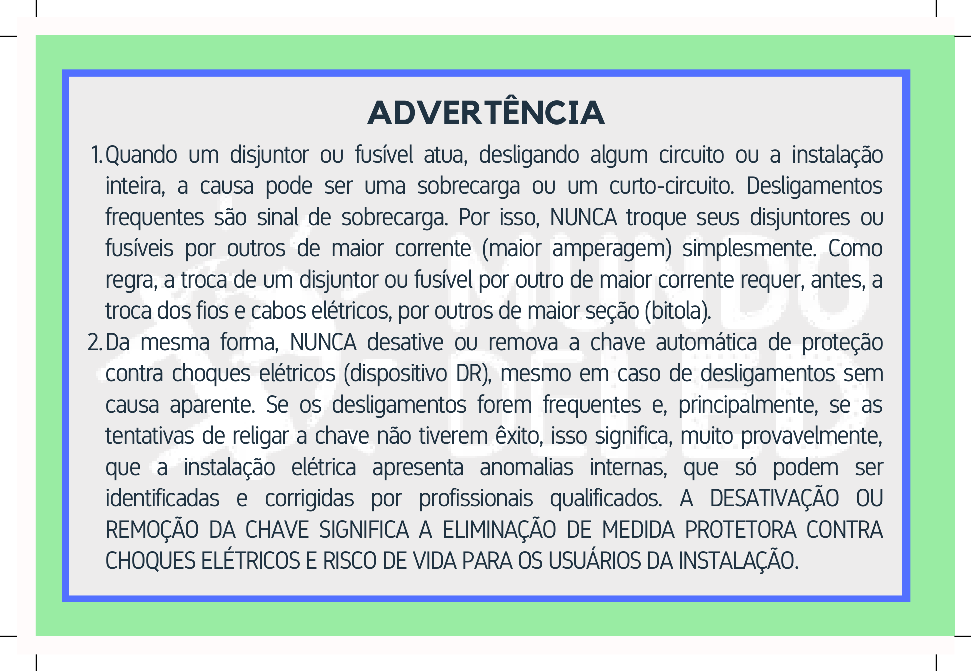
\includegraphics{image/EtiqAdvQD.pdf}
    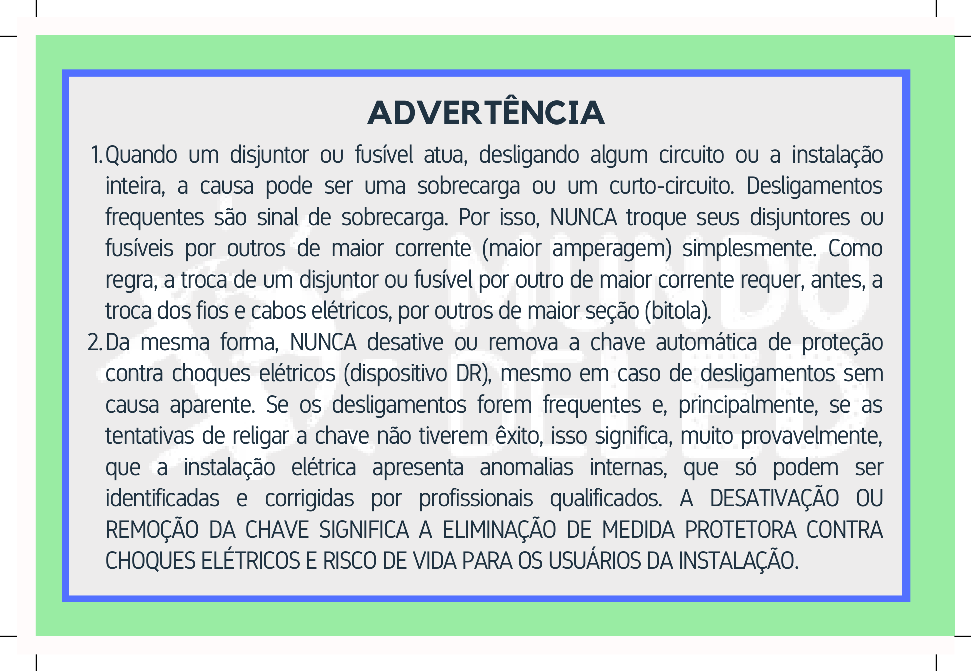
\includegraphics[scale=0.5]{image/EtiqAdvQD.pdf}
    \caption{Placa/ Adesivo de advertência para ser fixada no QD.}
    \label{fig:advQD}
\end{figure}

